\documentclass{article}%
\usepackage[T1]{fontenc}%
\usepackage[utf8]{inputenc}%
\usepackage{lmodern}%
\usepackage{textcomp}%
\usepackage{lastpage}%
\usepackage[head=40pt,margin=0.5in,bottom=0.6in]{geometry}%
\usepackage{graphicx}%
%
\title{\textbf{CIDH pide ir a Venezuela para evaluar situación de los derechos humanos}}%
\author{EFE}%
\date{04/10/2018}%
%
\begin{document}%
\normalsize%
\maketitle%
\textbf{URL: }%
http://www.eluniversal.com/politica/22353/la{-}cidh{-}pide{-}ir{-}a{-}venezuela{-}para{-}evaluar{-}la{-}situacion{-}de{-}derechos{-}humanos\newline%
%
\textbf{Periodico: }%
EU, %
ID: %
22353, %
Seccion: %
politica\newline%
%
\textbf{Palabras Claves: }%
NO\_TIENE\newline%
%
\textbf{Derecho: }%
18, %
Otros Derechos: %
, %
Sub Derechos: %
\newline%
%
\textbf{EP: }%
NO\newline%
\newline%
%
\textbf{\textit{La Comisión, órgano autónomo de la OEA lleva solicitando durante siete años permiso a Venezuela para visitar su territorio,  sin que haya habido una respuesta de momento}}%
\newline%
\newline%
%
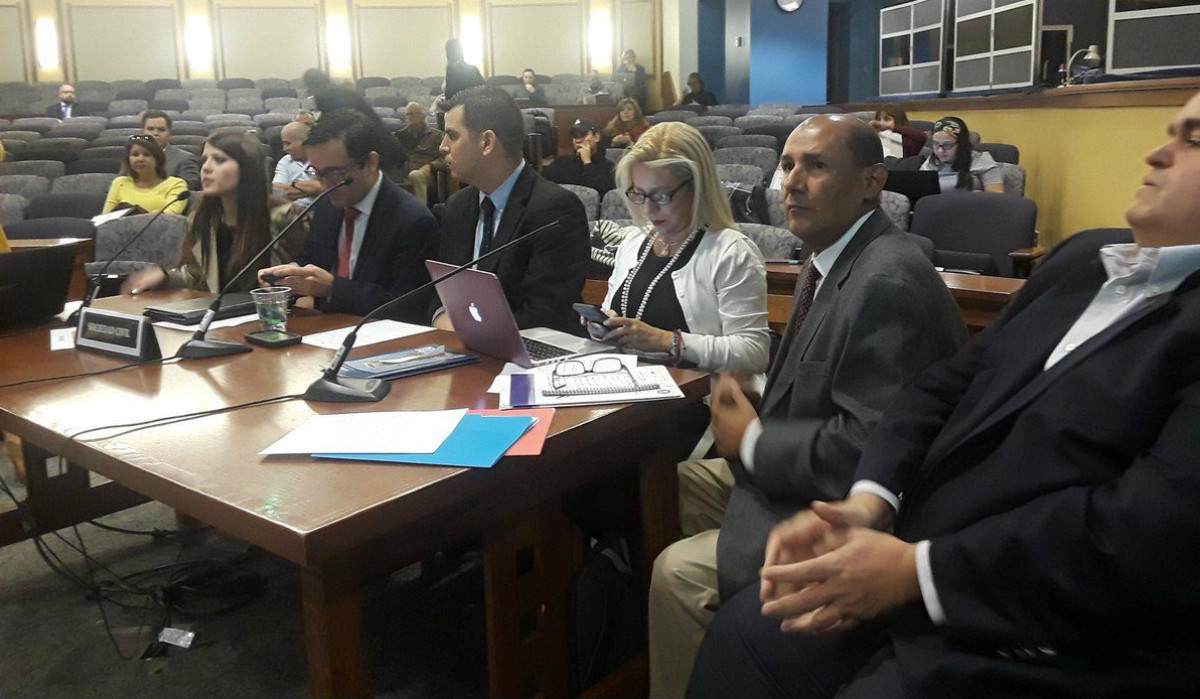
\includegraphics[width=300px]{130.jpg}%
\newline%
%
Boulder.{-}La Comisión Interamericana de Derechos Humanos (CIDH) volvió este jueves a pedir permiso al Estado de Venezuela para visitar el país con el objetivo evaluar la situación, especialmente en el ámbito de la atención médica y el acceso a alimentos.%
\newline%
%
La relatora de la CIDH para Derechos Económicos, Sociales, Culturales y Ambientales, Soledad García Muñoz, formuló esa petición para examinar la situación de los derechos humanos en territorio venezolano durante una audiencia en el marco del 169 periodo de sesiones del organismo, que se celebra en la Universidad de Colorado, en Boulder (EEUU), García Muñoz expresó "inquietud" por la situación en Venezuela y puso la CIDH a disposición del Ejecutivo para asistencia técnica.%
\newline%
%
La Comisión, órgano autónomo de la Organización de Estados Americanos (OEA), lleva solicitando durante siete años permiso a Venezuela para visitar su territorio, la última vez en agosto junto a representantes de Naciones Unidas, sin que haya habido una respuesta de momento.%
\newline%
%
Están previstas otras dos sesiones: una convocada por iniciativa propia por la CIDH para estudiar las condiciones de las personas privadas de libertad en el "contexto de la crisis política", y otra para analizar la situación humanitaria y los "mecanismos de control social" en Venezuela, según figura en el calendario.%
\newline%
%
Entre el público había hoy varios ciudadanos venezolanos, entre ellos un joven que sostenía una pancarta con la bandera venezolana y el lema en ingles "Freedom for Venezuela" (Libertad para Venezuela).%
\newline%
%
Venezuela ha perdido más del 40 \% de su Producto Interior Bruto (PIB) en los últimos cuatro años y registra una inflación disparada, que se calcula que alcance el 1.000.000 \% este año, según datos del Fondo Monetario Internacional (FMI).%
\newline%
%
La ONU estima que hasta junio de este año 2,3 millones de venezolanos han salido de su país, principalmente con rumbo a Colombia, Ecuador, Perú, Brasil y Chile.%
\newline%
%
\end{document}